\documentclass{emulateapj}
%\documentclass[manuscript]{aastex}

\usepackage{graphicx}
\usepackage{subfigure}
\usepackage{verbatim}
\usepackage{natbib}
\usepackage{amsmath}
\bibliographystyle{apj}

\shorttitle{STAR-FORMING MAIN SEQUENCE GALAXIES AND THEIR MORPHOLOGY}
\shortauthors{WILLETT ET AL.}

\begin{document}

\title{The dependence of spiral disk morphology on the mass-star formation relation}

\author{Kyle Willett\altaffilmark{1}, Kevin Schawinski\altaffilmark{2}, etc.}

\altaffiltext{1}{School of Physics and Astronomy, University of Minnesota, Minneapolis, MN 55455, USA}
\altaffiltext{2}{Institute for Astronomy, Department of Physics, ETH Z\"urich, Wolfgang-Pauli-Strasse 16, CH-8093, Z\"urich, Switzerland}

%%%%%%%%%%%%
%%% ABSTRACT
%%%%%%%%%%%%

\begin{abstract}
We measure the mass-star formation relation in disk galaxies at $z<0.05$, using Galaxy Zoo morphologies to separate disk galaxies by their kiloparsec-scale spiral structure. We examine the number of arms, their average pitch angle, and the presence of a galactic bar, and show that both the slope and dispersion of the SFR-$M_{\rm stellar}$ relation is constant when varying all the above parameters. We interpret this as evidence that the spiral arms, which are imperfect reflections of the galaxy's current gravitational potential, are either fully independent of the basic quenching relation or are completely overwhelmed by the combination of outflows and feedback. The arrangement of the star formation can be changed (as demonstrated by the filling factor of the disk), but the system \emph{as a whole} regulates itself. 
\end{abstract}

\keywords{galaxies:mergers}

%%%%%%%%%%%%
%%% INTRODUCTION
%%%%%%%%%%%%

\section{Introduction} \label{sec-intro}

%ORIGINAL TEXT %Mass-SFR relationship is tight, universal, and redshift-dependent (many citations). We think this is the result of the balancing of cosmological inflows of gas from the halo and feedback mechanism \citep{bou10,lil13}. 

%NEW, COHERENT INTRO (hi there, @overheardonastroph!)
Observations at a range of redshifts have established that the star formation rate (SFR) of a galaxy is strongly correlated to its stellar mass ($M_{\rm stellar}$). This `main sequence' of star formation (MS) is nearly linear and at least at low redshift, has remarkably small scatter (refs). Recent observations of star-forming galaxies at high redshifts show that this main sequence remains out to high redshift with the normalisation of the main sequence shifting up so that galaxies of the same stellar mass have a higher SFR at high redshift (refs). The main sequence has been interpreted by \citet{bou10} and \citet{lil13} as the result of the balancing of inflows of cosmological gas and outflows due the feedback. Galaxies self-regulate to remain in a state of homeostasis as they convert baryons from gas to stars. 

As star-forming galaxies exhibit a wide range of physical appearances in optical images, we can ask the natural question of whether the specifics of this physical appearance, and its underlying dynamical processes, have any effect on this homeostasis and therefore the galaxy's location relative to the SFR-$M_{\rm stellar}$ relation. If the details of a galaxy's physical appearance are correlated with position relative to the main sequence, then the dynamical processes that give rise to them -- such as bar formation and spiral arm pitch angle -- are a fundamental aspect of the galaxy's regulatory mechanism. If on the other hand they are not correlated, then there are two options: either they are simply not relevant, or the regulatory mechanism overcomes them in virtually all circumstances. This would speak to the strength of the regulator.

In this paper, we use the Sloan Digital Sky Survey \citep{yor00,str02,aba09} in combination with the largest database of visual classifications of galaxy structure and morphology ever assembled from the Galaxy Zoo citizen science project \citep{lin08,lin11,wil13} to test whether galaxy structure affects their star formation properties.




%%%%%%%%%%%%
%%% Data
%%%%%%%%%%%%

\section{Data} \label{sec-data}

Description of Galaxy Zoo 2 \citep{wil13}. Stellar masses and SFR from MPA-JHU \citep{kau03a,bri04}. Select starforming galaxies using BPT diagram \citep{bal81} and the standard \citet{kau03} demarcation line. Spiral galaxies are selected according to the following vote and vote thresholds. 

Figure: example images of: 1-5 arms, plus arm tightness, plus barred vs. non-barred. 

Table~\ref{tbl-fits}: fits for all star forming galaxies and then split by different morphologies

\begin{table}
 \begin{tabular}{@{}lrcl}
 \hline
\multicolumn{1}{c}{Sample} &
\multicolumn{1}{c}{$\alpha$} &
\multicolumn{1}{c}{$\beta$} &
\multicolumn{1}{c}{$\sigma$} 
\\ 
\\ 
\hline
\hline						
%Main (original + extra)       & 273,783 & 43  & 17.0   \\     % 43.1
All star-forming galaxies  & & & \\
\hline
$N_{arms} = 1$ & & & \\
$N_{arms} = 2$ & & & \\
$N_{arms} = 3$ & & & \\
$N_{arms} = 4$ & & & \\
$N_{arms} = 5$ & & & \\
$N_{arms} = ?$ & & & \\
\hline
Tight & & & \\
Medium & & & \\
Loose & & & \\
\hline
Barred & & & \\
Unbarred & & & \\
\hline
 \end{tabular}
 \caption{Basic properties of the $M_\star-SFR$ linear fit for GZ2 star-forming galaxies. \label{tbl-fits}}
\end{table}

Figure~\ref{fig-number}: $M_\star-SFR$ for arm multiplicity \\
Figure~\ref{fig-winding}: $M_\star-SFR$ for pitch angle ($\phi$) \\
Figure~\ref{fig-bar}: $M_\star-SFR$ for barred vs unbarred \\

How many galaxies are there in the total sample? What is the mass, color, and redshift range?

%%%%%%%%%%%%
%%% RESULTS
%%%%%%%%%%%%

\section{Results} \label{sec-results}

\begin{figure*}
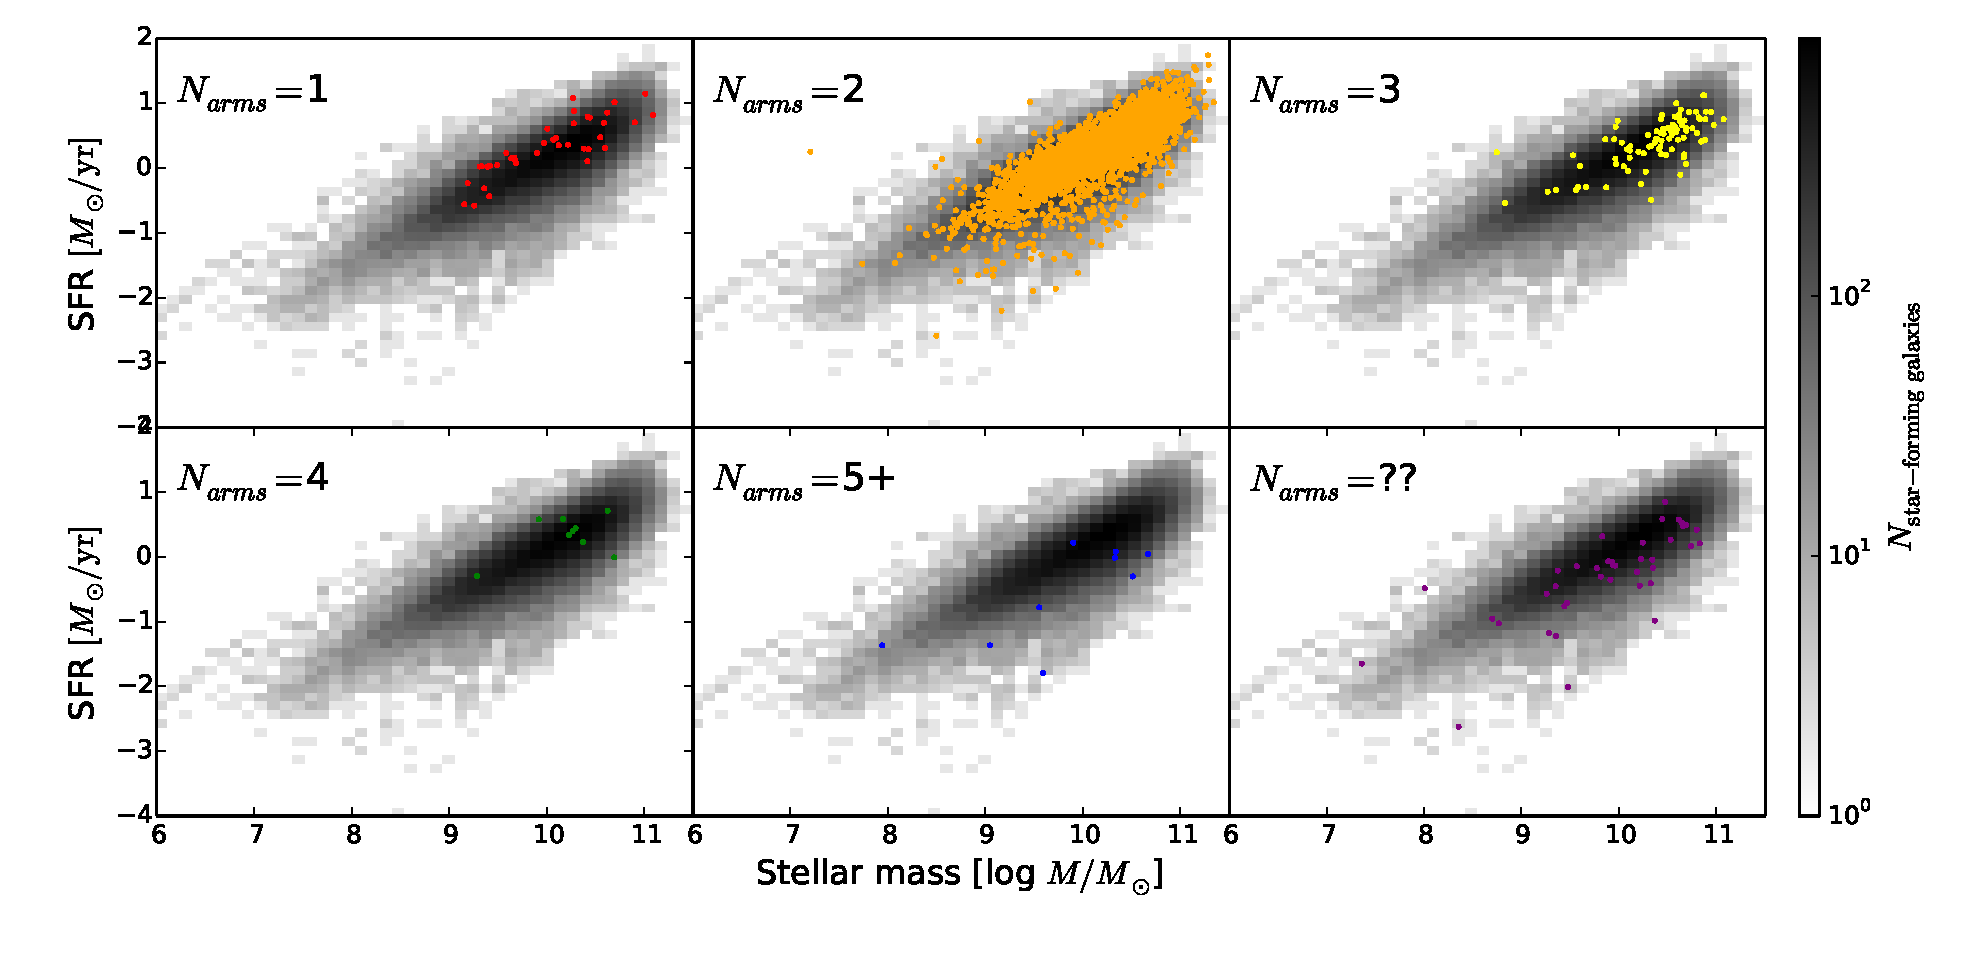
\includegraphics[angle=0,width=7.0in]{ms_arms_number.pdf}
\caption{Stellar mass vs. star formation rate for oblique disk galaxies in GZ2, split by the number of spiral arms. Both stellar mass and SFR are taken from the MPA-JHU catalog for DR7. 
\label{fig-number}}
\end{figure*}

\begin{figure*}
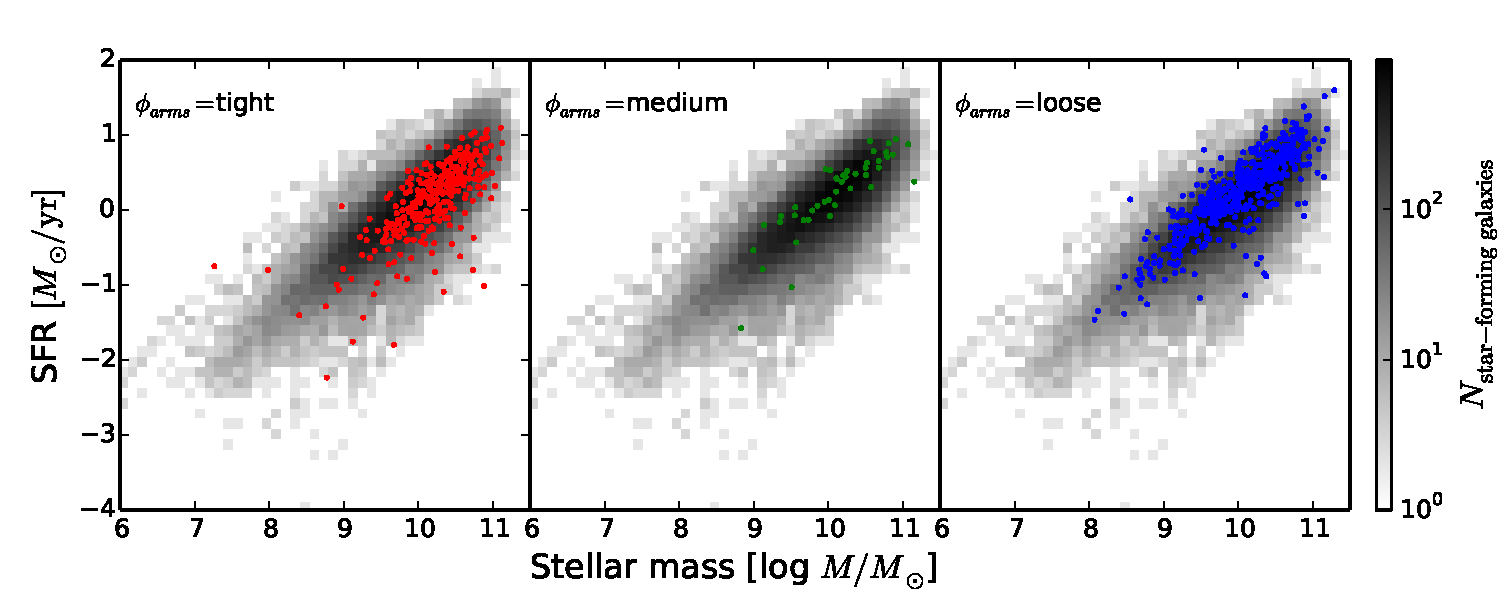
\includegraphics[angle=0,width=7.0in]{ms_arms_winding.pdf}
\caption{Stellar mass vs. star formation rate for oblique disk galaxies in GZ2, split by the relative pitch angle of the spiral arms. 
\label{fig-winding}}
\end{figure*}

\begin{figure*}
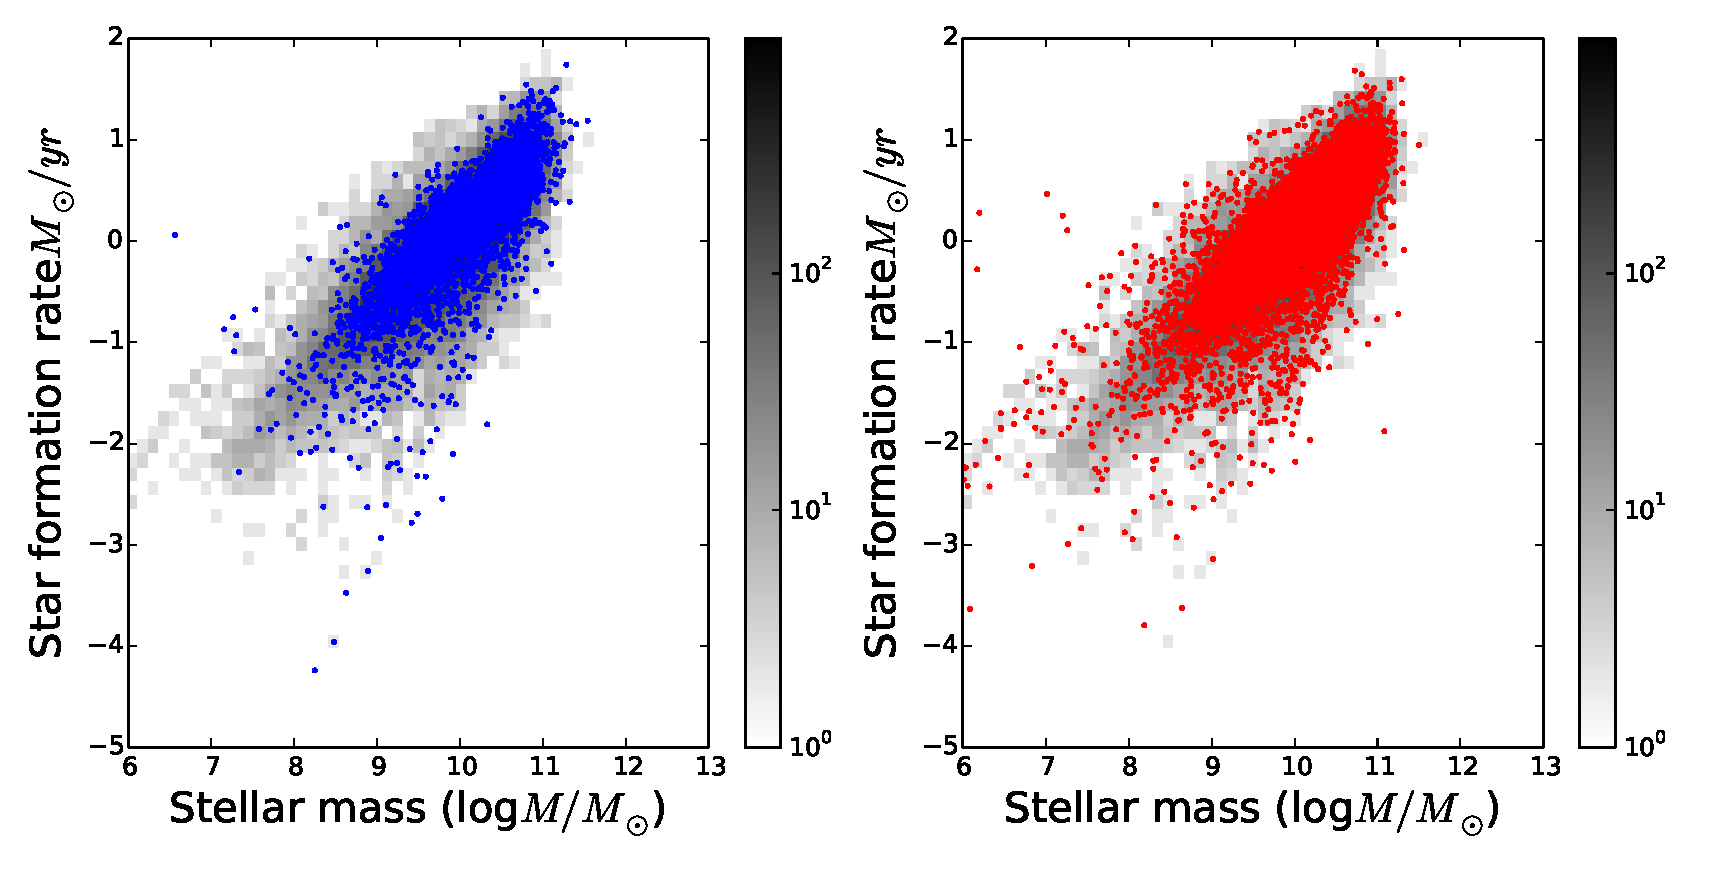
\includegraphics[angle=0,width=7.0in]{ms_bar.pdf}
\caption{Stellar mass vs. star formation rate for oblique disk galaxies in GZ2, split by the detection of a galactic bar. 
\label{fig-bar}}
\end{figure*}

List the fits to slope and intercept for the linear version of the M-SFR relation. Also look at dispersion. 

%%%%%%%%%%%%
%%% DISCUSSION
%%%%%%%%%%%%

\section{Discussion}\label{sec-discussion}

There is no significant difference between any of the morphological categories explored. Statistical test for how not different the categories are. 

This is interpreted as evidence that the regulation of the star formation rate is independent of the details of galactic structure as traced by the dynamics of the spiral arms. 

Conditional statements: if the situation above is true, then the following must apply. 

Point that has not been made before; self-regulated systems where you can move parts around, but the total amount must be conserved. Process as a result cannot be simply regulated locally - the whole system must know about the rate of regulation. What does this say about the minimum lifetime of the features as a dynamical timescale $\tau_{dyn}$? 

Connection between galaxy structure and quenching efficiency - \citet{oma14} found a simple dependence on $B/T$ for SDSS DR7 data. 

%%%%%%%%%%%%
%%% ACKNOWLEDGMENTS
%%%%%%%%%%%%

\acknowledgments

The data in this paper are the result of the efforts of the Galaxy~Zoo volunteers, without whom none of this work would be possible. Their efforts are individually acknowledged at \url{http://authors.galaxyzoo.org}. Please contact the authors to request access to research materials discussed in this paper. 

This research made use of TOPCAT, an interactive graphical viewer and editor for tabular data \citep{tay05}. 
%The development of Galaxy Zoo 2 was supported by The Leverhulme Trust. KWW and LFF would like to acknowledge support from the US National Science Foundation under grant DRL-0941610. CJL acknowledges support from the Science and Technology Facilities Council (STFC) Science in Society program. KS gratefully acknowledges support from Swiss National Science Foundation Grant PP00P2\_138979/1. TM acknowledges funding from the STFC ST/J500665/1. RCN was partially supported by STFC grant ST/K00090X/1. BDS acknowledges support from Worcester College, Oxford, and from the Oxford Martin School program on computational cosmology.

Funding for the SDSS and SDSS-II has been provided by the Alfred P. Sloan Foundation, the Participating Institutions, the National Science Foundation, the U.S. Department of Energy, the National Aeronautics and Space Administration, the Japanese Monbukagakusho, the Max Planck Society, and the Higher Education Funding Council for England. The SDSS website is \url{http://www.sdss.org/}.

The SDSS is managed by the Astrophysical Research Consortium for the Participating Institutions. The Participating Institutions are the American Museum of Natural History, Astrophysical Institute Potsdam, University of Basel, University of Cambridge, Case Western Reserve University, University of Chicago, Drexel University, Fermilab, the Institute for Advanced Study, the Japan Participation Group, Johns Hopkins University, the Joint Institute for Nuclear Astrophysics, the Kavli Institute for Particle Astrophysics and Cosmology, the Korean Scientist Group, the Chinese Academy of Sciences (LAMOST), Los Alamos National Laboratory, the Max-Planck-Institute for Astronomy (MPIA), the Max-Planck-Institute for Astrophysics (MPA), New Mexico State University, Ohio State University, University of Pittsburgh, University of Portsmouth, Princeton University, the United States Naval Observatory, and the University of Washington.

\clearpage

%%%%%%%%%%%%
%%% BIBLIOGRAPHY
%%%%%%%%%%%%

\bibliography{kwrefs}

\end{document}


